\documentclass[tikz]{standalone}
\input{figures/common/preamble}

\begin{document}
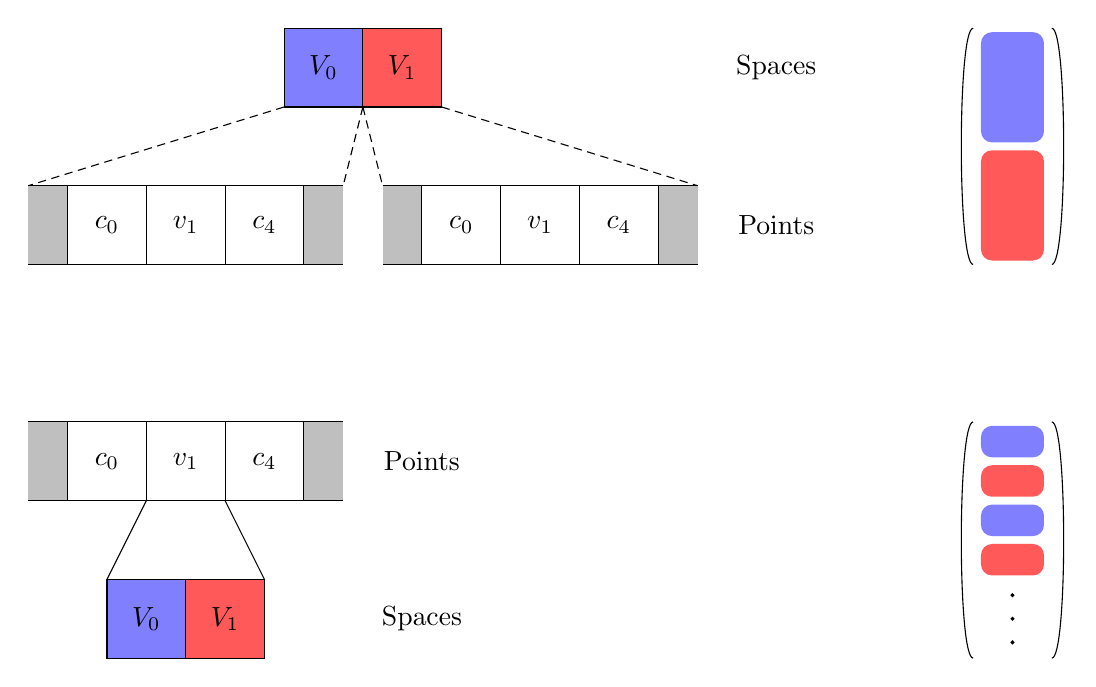
\begin{tikzpicture}[y=-1cm]

\newcommand{\mixedstylesetup}{%
  \tikzstyle{v0} = [fill=blue!50];
  \tikzstyle{v1} = [fill=red!65];
}
\tikzstyle{ptlabel} = [anchor=center, color=black, opacity=1]

\mixedstylesetup

\begin{scope}[xshift=3.25cm]
  \filldraw[v0,draw=black] (0,0) rectangle (1,1);
  \filldraw[v1,draw=black] (1,0) rectangle (2,1);
  \node[at={(.5,.5)}, ptlabel] {$V_0$};
  \node[at={(1.5,.5)}, ptlabel] {$V_1$};
\end{scope}

\begin{scope}[yshift=-2cm]
  \begin{scope}[xshift=0cm]
    \fill[lightgray] (0,0) rectangle (4,1);
    \filldraw[draw=black, fill=white] (0.5,0) rectangle (1.5,1);
    \filldraw[draw=black, fill=white] (1.5,0) rectangle (2.5,1);
    \filldraw[draw=black, fill=white] (2.5,0) rectangle (3.5,1);
    \node[at={(1,.5)}, ptlabel] {$c_0$};
    \node[at={(2,.5)}, ptlabel] {$v_1$};
    \node[at={(3,.5)}, ptlabel] {$c_4$};
    \draw (0,0) -- (4,0);
    \draw (0,1) -- (4,1);
  \end{scope}

  \begin{scope}[xshift=4.5cm]
    \fill[lightgray] (0,0) rectangle (4,1);
    \filldraw[draw=black, fill=white] (0.5,0) rectangle (1.5,1);
    \filldraw[draw=black, fill=white] (1.5,0) rectangle (2.5,1);
    \filldraw[draw=black, fill=white] (2.5,0) rectangle (3.5,1);
    \node[at={(1,.5)}, ptlabel] {$c_0$};
    \node[at={(2,.5)}, ptlabel] {$v_1$};
    \node[at={(3,.5)}, ptlabel] {$c_4$};
    \draw (0,0) -- (4,0);
    \draw (0,1) -- (4,1);
  \end{scope}
\end{scope}

\draw [densely dashed] (3.25,1) -- (0,2);
\draw [densely dashed] (4.25,1) -- (4,2);
\draw [densely dashed] (4.25,1) -- ({0+4.5},2);
\draw [densely dashed] (5.25,1) -- ({4+4.5},2);

\node [at={(9.5,.5)},anchor=center] {Spaces};
\node [at={(9.5,2.5)},anchor=center] {Points};

  \begin{scope}[xshift=12cm]
  \draw (0,0) .. controls (-.2,0) and (-.2,3) .. (0,3);
  \draw (1,0) .. controls (1.2,0) and (1.2,3) .. (1,3);
  \filldraw [v0,rounded corners,draw=none]
    (.1,.05) -- (.9,.05) -- (.9,1.45) -- (.1,1.45) -- cycle;
  \filldraw [v1,rounded corners,draw=none]
    (.1,1.55) -- (.9,1.55) -- (.9,2.95) -- (.1,2.95) -- cycle;
  \end{scope}

\begin{scope}[yshift=-5cm]
  \begin{scope}[xshift=0cm,yshift=0cm]
    \fill[lightgray] (0,0) rectangle (4,1);
    \filldraw[draw=black, fill=white] (0.5,0) rectangle (1.5,1);
    \filldraw[draw=black, fill=white] (1.5,0) rectangle (2.5,1);
    \filldraw[draw=black, fill=white] (2.5,0) rectangle (3.5,1);
    \node[at={(1,.5)}, ptlabel] {$c_0$};
    \node[at={(2,.5)}, ptlabel] {$v_1$};
    \node[at={(3,.5)}, ptlabel] {$c_4$};
    \draw (0,0) -- (4,0);
    \draw (0,1) -- (4,1);
  \end{scope}

  \begin{scope}[xshift=1cm, yshift=-2cm]
    \filldraw[v0,draw=black] (0,0) rectangle (1,1);
    \filldraw[v1,draw=black] (1,0) rectangle (2,1);
    \node[at={(.5,.5)}, ptlabel] {$V_0$};
    \node[at={(1.5,.5)}, ptlabel] {$V_1$};
  \end{scope}

  \draw (1.5,1) -- (1,2);
  \draw (2.5,1) -- (3,2);

  \node [at={(5,.5)},anchor=center] {Points};
  \node [at={(5,2.5)},anchor=center] {Spaces};
\end{scope}

\begin{scope}[yshift=-5cm,xshift=12cm]
      \tikzstyle{entry} = [rounded corners,draw=none];
      \tikzstyle{blue} = [v0,entry];
      \tikzstyle{red} = [v1,entry];
      \draw (0,0) .. controls (-.2,0) and (-.2,3) .. (0,3);
      \draw (1,0) .. controls (1.2,0) and (1.2,3) .. (1,3);
      \filldraw [blue] (.1,.05) -- (.9,.05) -- (.9,.45) -- (.1,.45) -- cycle;
      \filldraw [red] (.1,.55) -- (.9,.55) -- (.9,.95) -- (.1,.95) -- cycle;
      \filldraw [blue] (.1,1.05) -- (.9,1.05) -- (.9,1.45) -- (.1,1.45) -- cycle;
      \filldraw [red] (.1,1.55) -- (.9,1.55) -- (.9,1.95) -- (.1,1.95) -- cycle;
      % \filldraw [blue] (.1,2.05) -- (.9,2.05) -- (.9,2.45) -- (.1,2.45) -- cycle;
      % \filldraw [red] (.1,2.55) -- (.9,2.55) -- (.9,2.95) -- (.1,2.95) -- cycle;
      % ellipsis
      \filldraw [fill=black] (.5,2.2) circle (.5pt);
      \filldraw [fill=black] (.5,2.5) circle (.5pt);
      \filldraw [fill=black] (.5,2.8) circle (.5pt);
\end{scope}

\end{tikzpicture}
\end{document}
